\documentclass[10pt,a4paper]{article}
\usepackage[utf8]{inputenc}
\usepackage[english]{babel}
\usepackage{amsmath}
\usepackage{amsfonts}
\usepackage{amssymb}
\usepackage{graphicx}
\usepackage[margin=0.4in]{geometry}
%\usepackage[demo]{graphicx} % "demo" option just for this example
\usepackage{subcaption}
\usepackage{program}
\begin{document}

\section{The algorithm}

\begin{program}
\mbox{A reconstruction algorithm to generate complete trees from incomplete trees}
\BEGIN \\ %
 t = t_0
 \WHILE t < t_{present} \DO
  |Update | \lambda;\\
  |calculate | \sigma = \sum \lambda_j;\\
  |simulate | \Delta t =rexp(\sigma); \\
  \IF t+\Delta t < t_{i+1} \THEN
   t = t + \Delta t;\\
   |simulate extinction | t_{ext} = rexp(\mu_0);\\
   \IF t_{ext} + t < t_{present} \THEN
    |update tree with new speciated-extincted specie|
   \FI
  \FI
 t = |next branching time | t_{i} 
 \OD	 
\END
\end{program}


\section{Analysis}

The plots below shows scaterplots and histograms for each of the three parameter estimator: Each point in the histogram corresponds to one simulated tree; basically we simulate a tree, calculate the MLE of complete tree (x-axis), then drop extinct species, and performs the monte carlo framework using algorithm 1 inside it to get the MLE (y-axes) maximicing the join likelihood described in the apendix 

%\begin{figure}[!htb]
%\minipage{0.32\textwidth}

\begin{center}
\begin{figure}
  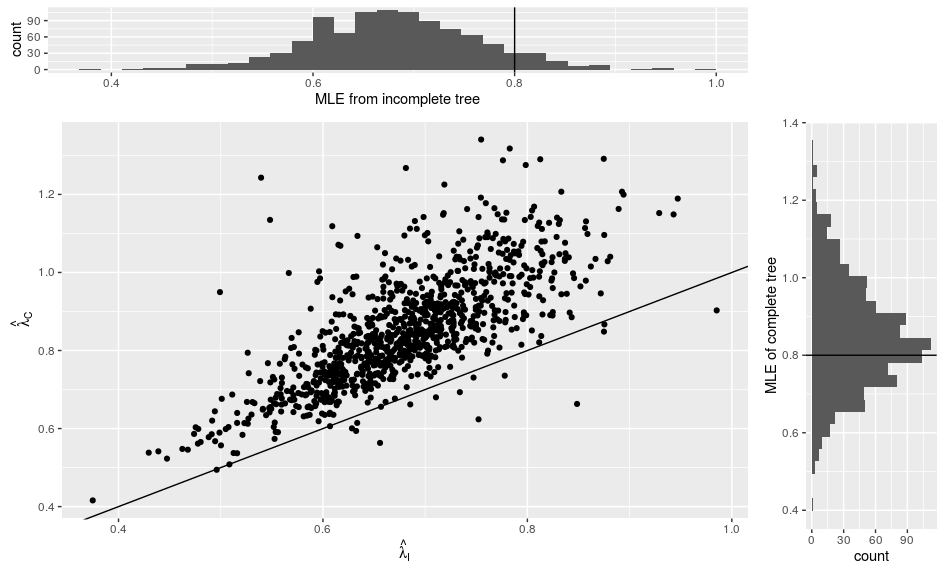
\includegraphics[scale=0.6]{lambda.png}
  \caption{Parameter estimation corresponding to $\lambda$}
\end{figure}
  \noindent\makebox[\linewidth]{\rule{\paperwidth}{0.4pt}}
%  \caption{A really Awesome Image}\label{fig:awesome_image1}
%\endminipage\hfill
%\minipage{0.32\textwidth}
  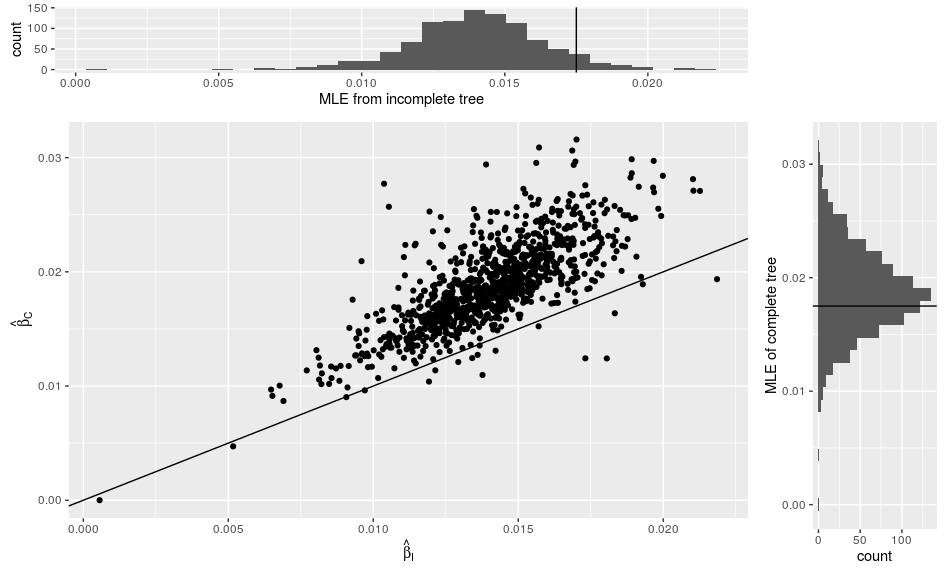
\includegraphics[scale=0.6]{beta.png}
  \noindent\makebox[\linewidth]{\rule{\paperwidth}{0.4pt}}
%  \caption{A really Awesome Image}\label{fig:awesome_image2}
%\endminipage\hfill
%\minipage{0.32\textwidth}%
  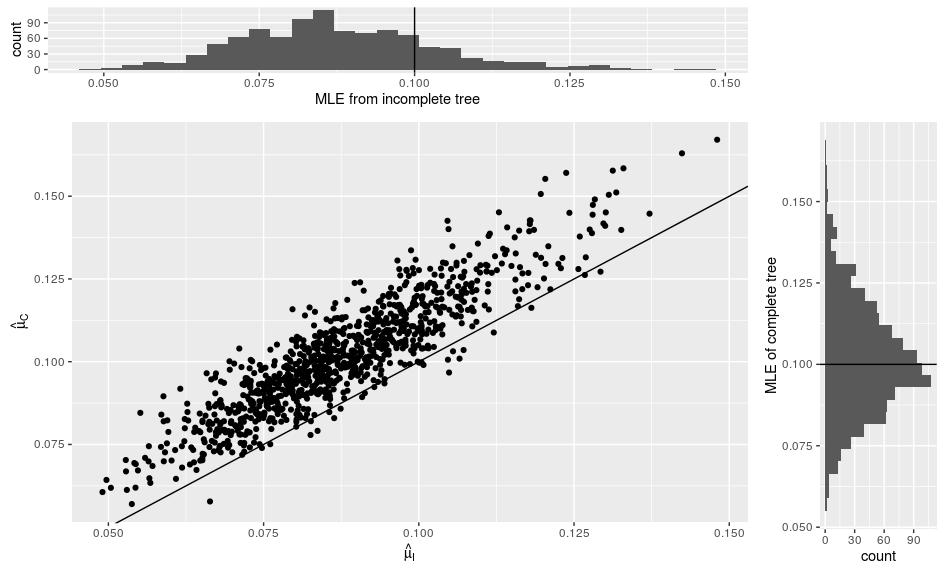
\includegraphics[scale=0.6]{mu.png}
  \noindent\makebox[\linewidth]{\rule{\paperwidth}{0.4pt}}
 % \caption{A really Awesome Image}\label{fig:awesome_image3}
%\endminipage
%\end{figure}
\end{center}

\section{Conclusions}



The reconstruction of tree using Algorithm 1 and the subsecuence ML estimation gives estimatos precise but not acurate, in other words biased estimators. This is the main potential reason of the non-estability of the EM algorithm (see example in appendix). This is maybe because the algorithm is generating less new species (figuras de los ltt plots y comparacion del numero de nuevas especies), 
To overcome this issue I see two posible ways: 

\begin{itemize}

	\item Work with algorithm 1 and use statistical tools to overcome the unbiased problem
	\item Search for an alternative to algorithm 1, it should makes slyghly more species

\end{itemize}

\section{Appendix 1. General way for a multi-trees approach}


Let $S=(s_1,...,s_m)$ be a set of trees and $ \mathcal{L} = (l_1(\theta),...,l_m(\theta))$ the set of log-likelihood functions of $S$. \\

Then 

$$ l_j(\theta) = \displaystyle\sum_{i=1}^{N_j} - \sigma_{i,j} t_{i,j}+log(\rho_{i,j}) $$
where $N_j$ is the number of branching times of the $j-$tree, $t_{i,j}$ is the $i^{th}$ branching time of the $j$-tree and $\sigma_{i,j}$ and $\rho_{i,j}$ are functions of $\lambda_{i,j}(\theta)$ and $\mu_{i,j}(\theta)$, which are the speciation and extinction rates of the species of the tree $j$ at time $t_{i,j}$ as described in previous reports.\\

In order to solve the E-step on the EM rutine, under the monte-carlo approach, we need to calculate 

$$ l(\theta) = \displaystyle\sum_{j = 1}^m l_j(\theta) $$

the M-step corresponds to find $\max_{\theta} l(\theta) $.

\subsection{Diversity dependence model}

 
As described previously, we define 

$$ l_j(\theta) = log(L(\theta \| s_j)) $$

in the case of diversity-dependence, where we have \\

$\sigma_{i,j} = n_{i,j}\lambda -\beta n_{i,j}^2+n_{i,j}\mu$ \\
$\rho_{i,j} = E_{i,j}(\lambda-\beta n_{i,j})+(1-E_{i,j})\mu$ \\

Thus,

$$ l_j((\lambda,\beta,\mu)) = \displaystyle\sum_{i=1}^{N_j} -t_{i,j}[n_{i,j}\lambda-n_{i,j}^2 \beta - n_{i,j}\mu]+log(E_{i,j}(\lambda-\beta n_{i,j})+(1-E_{i,j})\mu)$$

Moreover, 

$$ l(\theta) = \displaystyle\sum_{j=1}^m \displaystyle\sum_{i=1}^{N_j} -t_{i,j}[n_{i,j}\lambda -n_{i,j}^2 \beta + n_{i,j} \mu] + log(E_{i,j}(\lambda-\beta n_{i,j})+(1-E_{i,j})\mu) $$ 

where, as in the case of 1 single tree, we can find an analytical solution for the parameter $\mu$

$$ \mu = \frac{\displaystyle\sum_{j=1}^m \displaystyle\sum_{i=1}^{N_j}(1-E_{i,j})}{\displaystyle\sum_{j=1}^m \displaystyle\sum_{i=1}^{N_j} t_{i,j}n_{i,j}} $$

and the other two parameters might be calculated under the same framework of the single tree case. 

%\section*{The algorithm}


\section{EM Example (seed 7)}

EM example below. 

\begin{table}[h!]
\centering
\caption{EM iterations}
\label{my-label}
\begin{tabular}{l|llll}
it & $\lambda$ & $\beta$ & $\mu$ & $K$ \\ \hline
1  & 1.43      & 0.015   & 0.55  & 58  \\
2  & 1.09      & 0.01    & 0.43  & 66  \\
3  & 0.85      & 0.007   & 0.36  & 70  \\
4  & 0.71      & 0.0055  & 0.32  & 71  \\
5  & 0.63      & 0.005   & 0.28  & 69  \\
6  & 0.61      & 0.0055  & 0.25  & 65  \\
7  & 0.59      & 0.006   & 0.23  & 61  \\
8  & 0.57      & 0.0065  & 0.20  & 57  \\
9  & 0.55      & 0.007   & 0.18  & 53  \\
10 & 0.53      & 0.0075  & 0.15  & 50  \\
11 & 0.51      & 0.008   & 0.13  & 47  \\
12 & 0.51      & 0.009   & 0.11  & 44  \\
13 & 0.51      & 0.0095  & 0.10  & 43  \\
14 & 0.49      & 0.0095  & 0.08  & 43  \\
15 & 0.47      & 0.0095  & 0.07  & 42  \\
16 & 0.45      & 0.0095  & 0.06  & 41  \\
17 & 0.43      & 0.0095  & 0.06  & 39  \\
18 & 0.41      & 0.009   & 0.05  & 40  \\
19 & 0.43      & 0.01    & 0.04  & 39  \\
20 & 0.39      & 0.009   & 0.03  & 40  \\
21 & 0.39      & 0.009   & 0.03  & 40  \\
22 & 0.37      & 0.0085  & 0.03  & 40  \\
23 & 0.35      & 0.008   & 0.02  & 41  \\
24 & 0.37      & 0.009   & 0.02  & 39  \\
25 & 0.37      & 0.009   & 0.01  & 39  \\
26 & 0.37      & 0.009   & 0.01  & 40  \\
27 & 0.35      & 0.0085  & 0.01  & 40  \\
28 & 0.35      & 0.0085  & 0.01  & 40  \\
29 & 0.35      & 0.0085  & 0.01  & 40  \\
30 & 0.35      & 0.0085  & 0.01  & 40 
\end{tabular}
\end{table}
\end{document}